\chapter{Sentiment Analysis}

\newthought{Sentiment analysis is useful in many different situations.} It can be used to explore brand sentiment, observe story arcs, recognize hate speech, and so on. Orange uses simple lexicon-based methods to compute the sentiment of the text.

\vspace{-0.2cm}
\begin{figure*}[h]
  \centering
  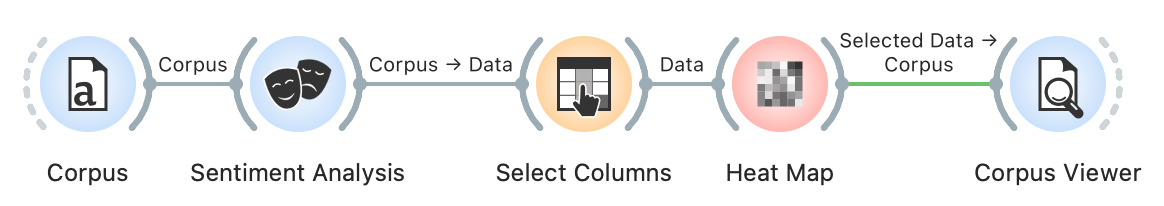
\includegraphics[width=0.9\linewidth]{workflow.png}%
  \caption{$\;$}
\end{figure*}
\vspace{-0.3cm}

Sentiment scores are computed in the \widget{Sentiment Analysis} widget. We will use the default \emph{Vader} method, but feel free to try the others. In \widget{Select Columns}, we will keep only the sentiment scores and put all the other features in meta attributes.

\begin{figure*}[h]
    \centering
    \infinitewidthbox{
      \stackinset{r}{-0.4\linewidth}{t}{+0.15\linewidth}
      {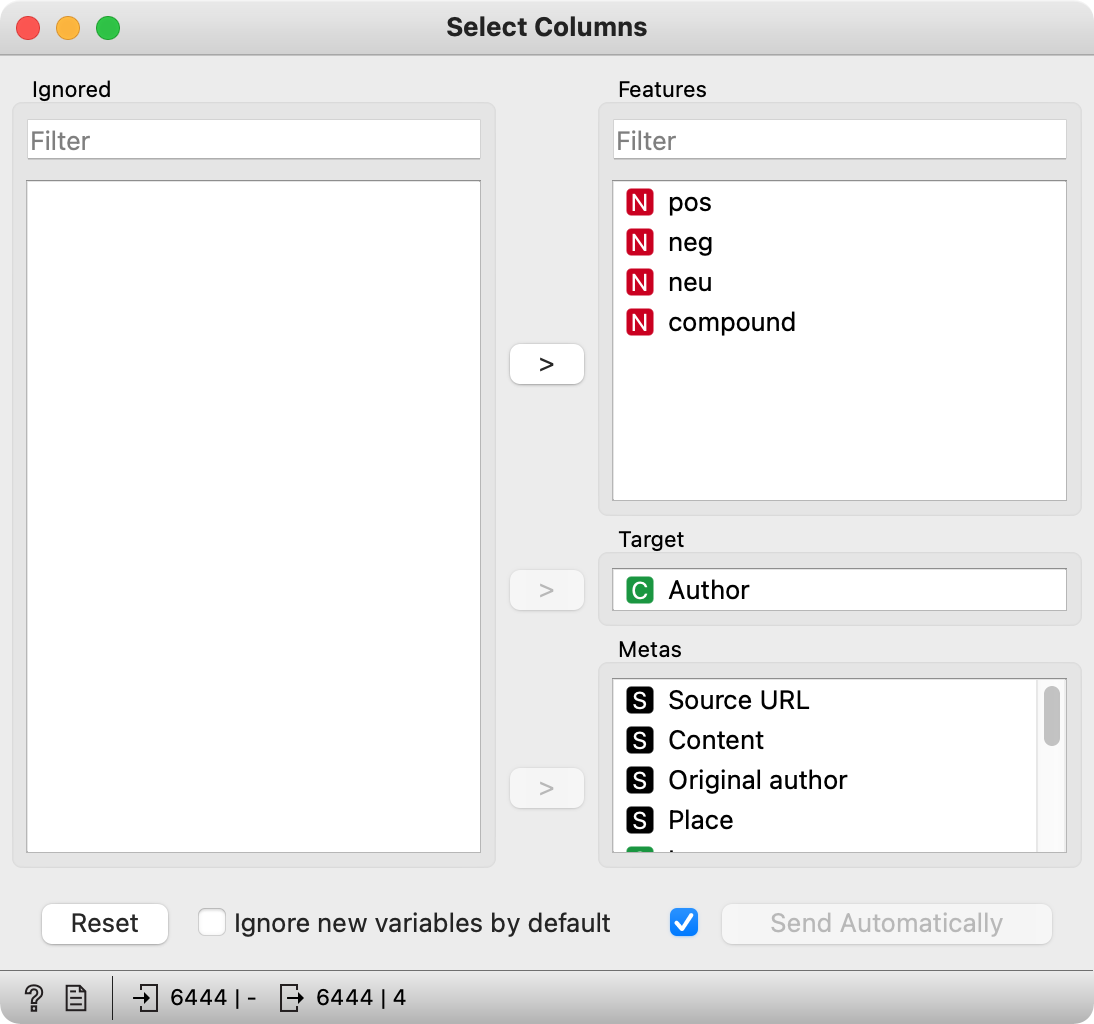
\includegraphics[scale=0.45]{select-columns.png}}
      {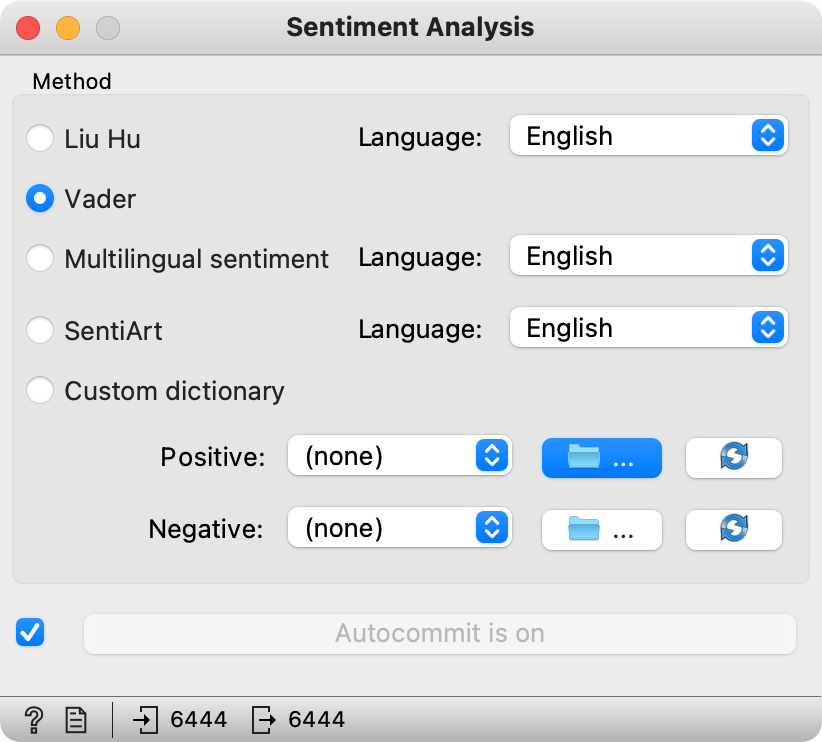
\includegraphics[scale=0.45]{sentiment-analysis.png}}
      \hspace{6cm}
      }
    \caption{$\;$}
\end{figure*}

A nice visualization for observing several numeric values at once is \widget{Heat Map}. Heat map shows documents in rows and attributes in columns, with the color of the field corresponding to its value. In this case, high values are yellow/white and low values are blue.

\begin{wrapfigure}{o}{1\textwidth}
    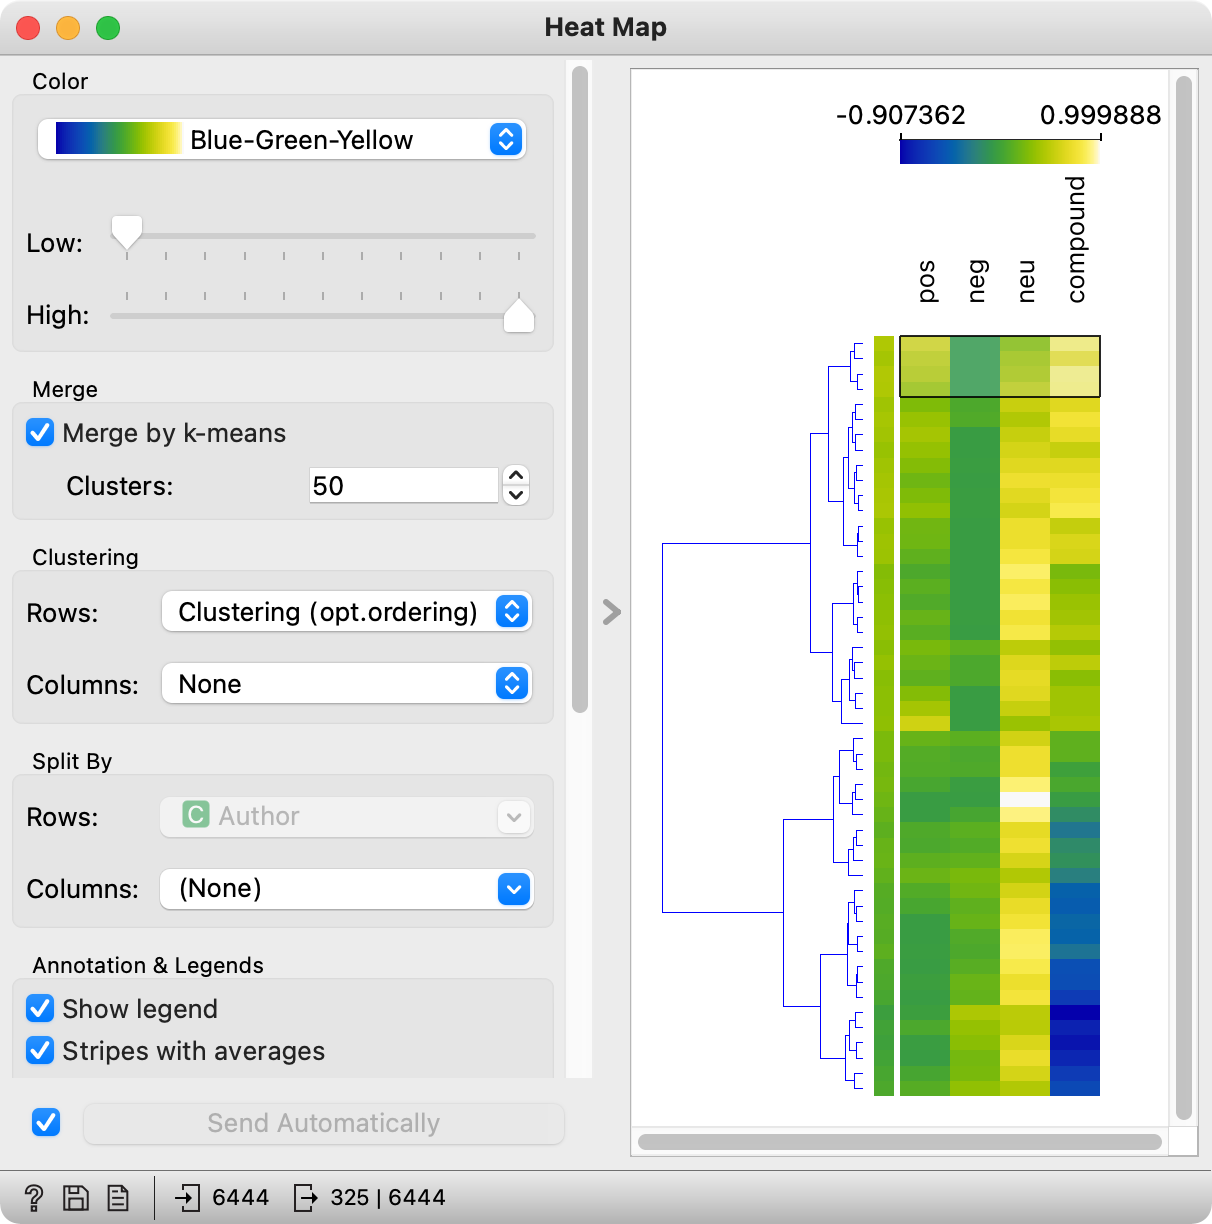
\includegraphics[scale=0.45]{heat-map.png}
    \caption{$\;$}
\end{wrapfigure}

But our data is completely unorganized and it is difficult to make sense of the visualization. Hence we will use some tricks to make it interpretable. First, we will join similar rows into a single row. We will do this with k-Means and keep only 50 rows.

Now, our visualization is much more compact. But preferrably, we would sort the rows in some logical order. For this, we will use \emph{Clustering (opt. ordering)} setting. It will use hierarchical clustering to put similar rows together and optimally place the leaves of the dendrogram.

The visualization is finally interpretable. At the top, we see positive documents, while in the bottom, the negative ones. Select the most positive documents by selecting the top leaf of the dendrogram. Then, observe the output in \widget{Corpus Viewer}.

Looks like our selection indeed contains positive tweets!

\vspace{-0.2cm}
\begin{figure*}[h]
  \centering
  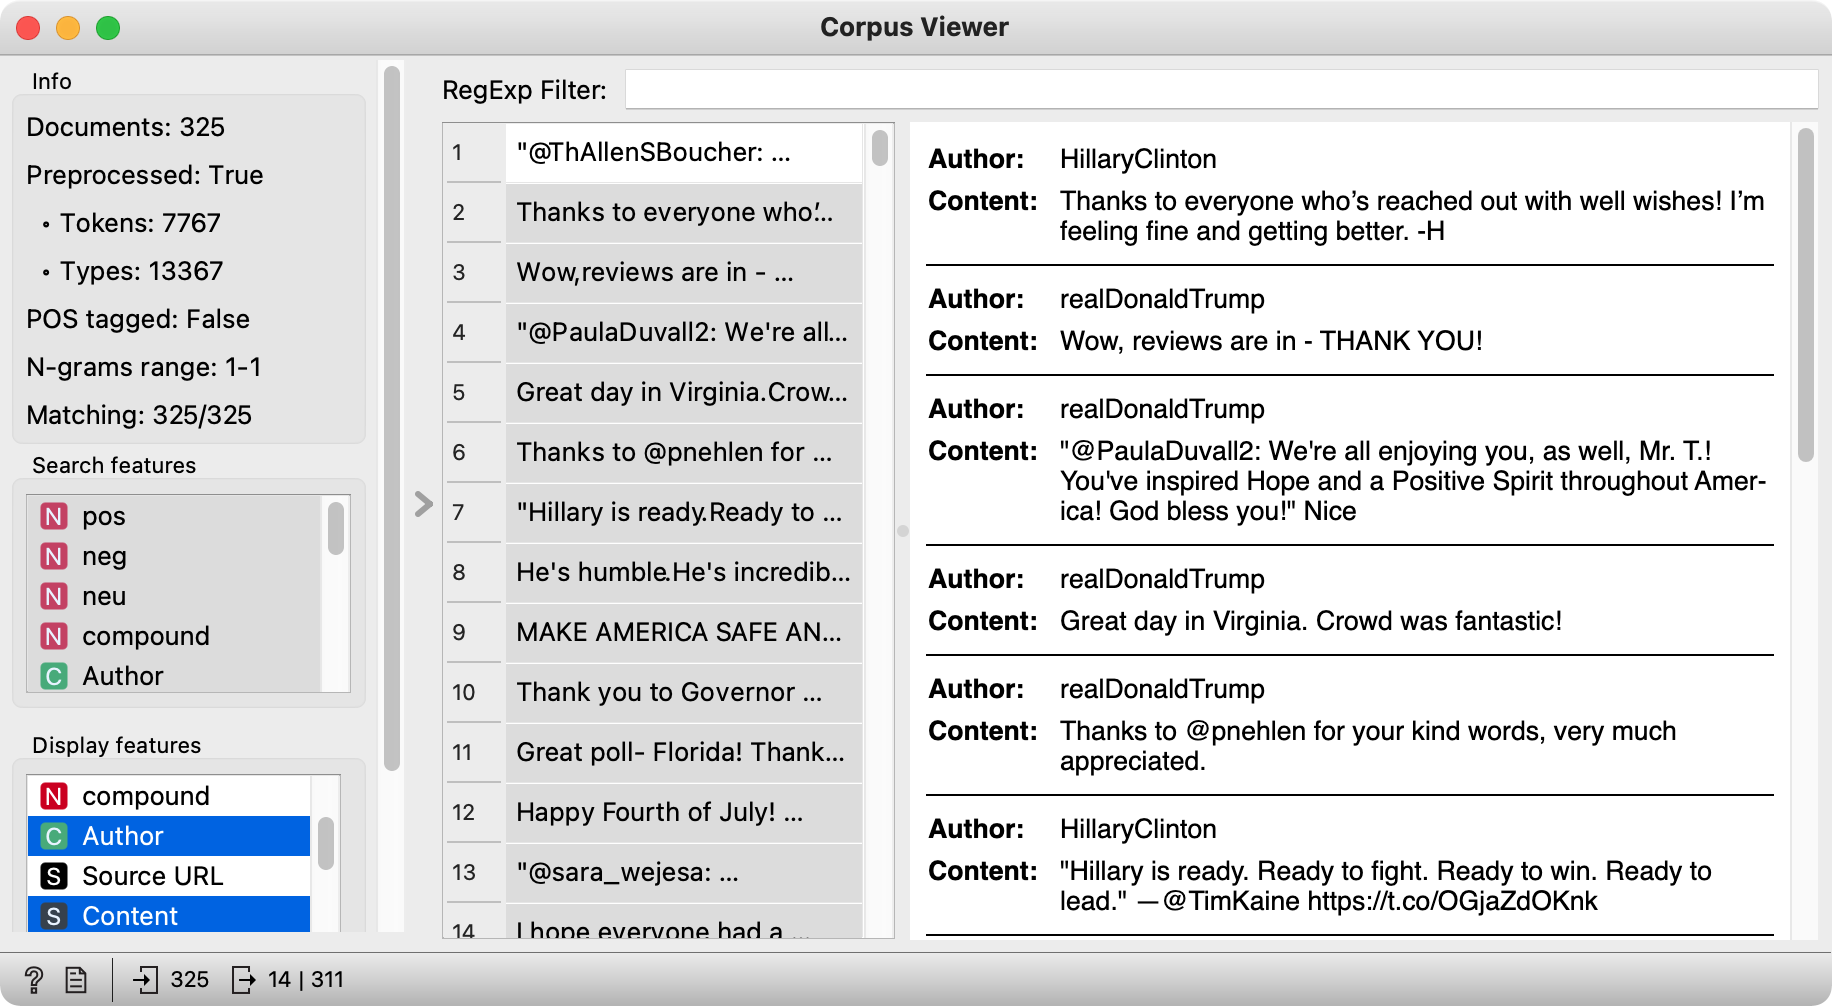
\includegraphics[width=\linewidth]{corpus-viewer.png}%
  \caption{$\;$}
\end{figure*}
\vspace{-0.3cm}
